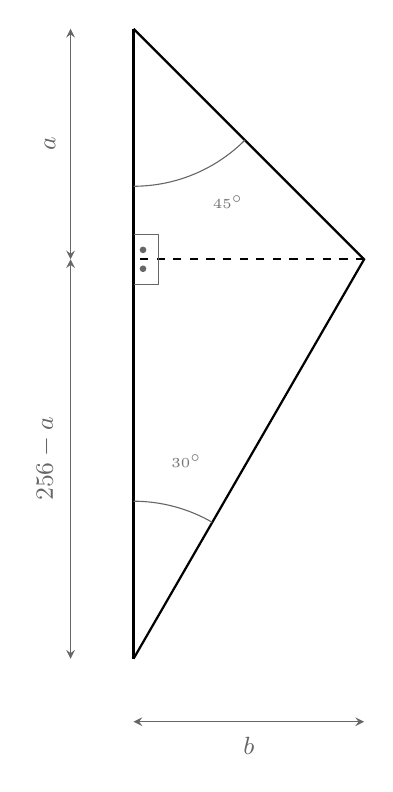
\begin{tikzpicture}[
    scale=4,
    cota/.style={<->, >=stealth, thin, gray!80!black},
    chamada/.style={gray!60, thin, dashed}
]
    % Coordenadas
    \coordinate (A) at (0, 0);
    \coordinate (D) at (0, 2);
    \coordinate (P1) at (0.732, 1.268);
    \coordinate (H) at (0, 1.268); % Ponto do corte na borda vertical

    % Desenho do Triângulo 1
    \draw[thick] (D) -- (A);                  % Borda livre da esquerda
    \draw[thick] (A) -- (P1) -- (D);          % Linhas de charneira
    \draw[thick,dashed] (P1) -- (H);          % Linha de corte/altura

    % Símbolos de Ângulo Reto (90°) na interseção da linha tracejada
    \draw[thin, gray!80!black] (0, 1.268-0.08) -- (0.08, 1.268-0.08) -- (0.08, 1.268);
    \fill[gray!80!black] (0.03, 1.268-0.03) circle (0.3pt);
    
    \draw[thin, gray!80!black] (0, 1.268+0.08) -- (0.08, 1.268+0.08) -- (0.08, 1.268);
    \fill[gray!80!black] (0.03, 1.268+0.03) circle (0.3pt);

    % Indicações dos Ângulos
    \draw[thin, gray!80!black] (0, 1.5) arc (270:315:0.5);
    \node[font=\tiny, gray!90!black] at (0.3, 1.45) {$45^\circ$};

    % Canto inferior (A): 30° da diagonal (60°) até a reta vertical (90°)
    \draw[thin, gray!80!black] (60:0.5) arc (60:90:0.5);
    \node[font=\tiny, gray!90!black] at (75:0.65) {$30^\circ$};

    % --- EIXO DE COTA HORIZONTAL (Largura x1) ---
    \def\offsetH{0.2}
    %\draw[chamada] (A) -- (0, -\offsetH);
    %\draw[chamada] (P1) -- (0.732, -\offsetH);
    \draw[cota] (0, -\offsetH) -- (0.732, -\offsetH)
        node[midway, below=2pt, font=\small] {$b$};

    % --- EIXOS DE COTA VERTICAIS (Alturas) ---
    \def\offsetV{0.2}
    %\draw[chamada] (A) -- (-\offsetV, 0);
    %\draw[chamada] (H) -- (-\offsetV, 1.268);
    %\draw[chamada] (D) -- (-\offsetV, 2);

    % Altura do trecho inferior
    \draw[cota] (-\offsetV, 0) -- (-\offsetV, 1.268)
        node[midway, left=2pt, font=\small, rotate=90, anchor=south] {$256-a$};

    % Altura do trecho superior
    \draw[cota] (-\offsetV, 1.268) -- (-\offsetV, 2)
        node[midway, left=2pt, font=\small, rotate=90, anchor=south] {$a$};

\end{tikzpicture}